% Options for packages loaded elsewhere
% Options for packages loaded elsewhere
\PassOptionsToPackage{unicode}{hyperref}
\PassOptionsToPackage{hyphens}{url}
\PassOptionsToPackage{dvipsnames,svgnames,x11names}{xcolor}
%
\documentclass[
  russian,
]{article}
\usepackage{xcolor}
\usepackage[top=20mm,left=20mm,right=20mm,bottom=20mm]{geometry}
\usepackage{amsmath,amssymb}
\setcounter{secnumdepth}{5}
\usepackage{iftex}
\ifPDFTeX
  \usepackage[T1]{fontenc}
  \usepackage[utf8]{inputenc}
  \usepackage{textcomp} % provide euro and other symbols
\else % if luatex or xetex
  \usepackage{unicode-math} % this also loads fontspec
  \defaultfontfeatures{Scale=MatchLowercase}
  \defaultfontfeatures[\rmfamily]{Ligatures=TeX,Scale=1}
\fi
\usepackage{lmodern}
\ifPDFTeX\else
  % xetex/luatex font selection
  \setmainfont[]{Times New Roman}
  \setsansfont[]{Arial}
  \setmonofont[]{Courier New}
\fi
% Use upquote if available, for straight quotes in verbatim environments
\IfFileExists{upquote.sty}{\usepackage{upquote}}{}
\IfFileExists{microtype.sty}{% use microtype if available
  \usepackage[]{microtype}
  \UseMicrotypeSet[protrusion]{basicmath} % disable protrusion for tt fonts
}{}
\makeatletter
\@ifundefined{KOMAClassName}{% if non-KOMA class
  \IfFileExists{parskip.sty}{%
    \usepackage{parskip}
  }{% else
    \setlength{\parindent}{0pt}
    \setlength{\parskip}{6pt plus 2pt minus 1pt}}
}{% if KOMA class
  \KOMAoptions{parskip=half}}
\makeatother
% Make \paragraph and \subparagraph free-standing
\makeatletter
\ifx\paragraph\undefined\else
  \let\oldparagraph\paragraph
  \renewcommand{\paragraph}{
    \@ifstar
      \xxxParagraphStar
      \xxxParagraphNoStar
  }
  \newcommand{\xxxParagraphStar}[1]{\oldparagraph*{#1}\mbox{}}
  \newcommand{\xxxParagraphNoStar}[1]{\oldparagraph{#1}\mbox{}}
\fi
\ifx\subparagraph\undefined\else
  \let\oldsubparagraph\subparagraph
  \renewcommand{\subparagraph}{
    \@ifstar
      \xxxSubParagraphStar
      \xxxSubParagraphNoStar
  }
  \newcommand{\xxxSubParagraphStar}[1]{\oldsubparagraph*{#1}\mbox{}}
  \newcommand{\xxxSubParagraphNoStar}[1]{\oldsubparagraph{#1}\mbox{}}
\fi
\makeatother


\usepackage{longtable,booktabs,array}
\newcounter{none} % for unnumbered tables
\usepackage{calc} % for calculating minipage widths
% Correct order of tables after \paragraph or \subparagraph
\usepackage{etoolbox}
\makeatletter
\patchcmd\longtable{\par}{\if@noskipsec\mbox{}\fi\par}{}{}
\makeatother
% Allow footnotes in longtable head/foot
\IfFileExists{footnotehyper.sty}{\usepackage{footnotehyper}}{\usepackage{footnote}}
\makesavenoteenv{longtable}
\usepackage{graphicx}
\makeatletter
\newsavebox\pandoc@box
\newcommand*\pandocbounded[1]{% scales image to fit in text height/width
  \sbox\pandoc@box{#1}%
  \Gscale@div\@tempa{\textheight}{\dimexpr\ht\pandoc@box+\dp\pandoc@box\relax}%
  \Gscale@div\@tempb{\linewidth}{\wd\pandoc@box}%
  \ifdim\@tempb\p@<\@tempa\p@\let\@tempa\@tempb\fi% select the smaller of both
  \ifdim\@tempa\p@<\p@\scalebox{\@tempa}{\usebox\pandoc@box}%
  \else\usebox{\pandoc@box}%
  \fi%
}
% Set default figure placement to htbp
\def\fps@figure{htbp}
\makeatother



\ifLuaTeX
\usepackage[bidi=basic,shorthands=off,provide=*]{babel}
\else
\usepackage[bidi=default,shorthands=off,provide=*]{babel}
\fi
\ifPDFTeX
\else
\babelfont{rm}[]{Times New Roman}
\fi
\ifLuaTeX
  \usepackage{selnolig} % disable illegal ligatures
\fi


\setlength{\emergencystretch}{3em} % prevent overfull lines

\providecommand{\tightlist}{%
  \setlength{\itemsep}{0pt}\setlength{\parskip}{0pt}}



 


\makeatletter
\@ifpackageloaded{tcolorbox}{}{\usepackage[skins,breakable]{tcolorbox}}
\@ifpackageloaded{fontawesome5}{}{\usepackage{fontawesome5}}
\definecolor{quarto-callout-color}{HTML}{909090}
\definecolor{quarto-callout-note-color}{HTML}{0758E5}
\definecolor{quarto-callout-important-color}{HTML}{CC1914}
\definecolor{quarto-callout-warning-color}{HTML}{EB9113}
\definecolor{quarto-callout-tip-color}{HTML}{00A047}
\definecolor{quarto-callout-caution-color}{HTML}{FC5300}
\definecolor{quarto-callout-color-frame}{HTML}{acacac}
\definecolor{quarto-callout-note-color-frame}{HTML}{4582ec}
\definecolor{quarto-callout-important-color-frame}{HTML}{d9534f}
\definecolor{quarto-callout-warning-color-frame}{HTML}{f0ad4e}
\definecolor{quarto-callout-tip-color-frame}{HTML}{02b875}
\definecolor{quarto-callout-caution-color-frame}{HTML}{fd7e14}
\makeatother
\makeatletter
\@ifpackageloaded{caption}{}{\usepackage{caption}}
\AtBeginDocument{%
\ifdefined\contentsname
  \renewcommand*\contentsname{Содержание}
\else
  \newcommand\contentsname{Содержание}
\fi
\ifdefined\listfigurename
  \renewcommand*\listfigurename{Список Иллюстраций}
\else
  \newcommand\listfigurename{Список Иллюстраций}
\fi
\ifdefined\listtablename
  \renewcommand*\listtablename{Список Таблиц}
\else
  \newcommand\listtablename{Список Таблиц}
\fi
\ifdefined\figurename
  \renewcommand*\figurename{Рисунок}
\else
  \newcommand\figurename{Рисунок}
\fi
\ifdefined\tablename
  \renewcommand*\tablename{Таблица}
\else
  \newcommand\tablename{Таблица}
\fi
}
\@ifpackageloaded{float}{}{\usepackage{float}}
\floatstyle{ruled}
\@ifundefined{c@chapter}{\newfloat{codelisting}{h}{lop}}{\newfloat{codelisting}{h}{lop}[chapter]}
\floatname{codelisting}{Список}
\newcommand*\listoflistings{\listof{codelisting}{Список Каталогов}}
\makeatother
\makeatletter
\makeatother
\makeatletter
\@ifpackageloaded{caption}{}{\usepackage{caption}}
\@ifpackageloaded{subcaption}{}{\usepackage{subcaption}}
\makeatother
\usepackage{bookmark}
\IfFileExists{xurl.sty}{\usepackage{xurl}}{} % add URL line breaks if available
\urlstyle{same}
\hypersetup{
  pdftitle={Задачи по Эконометрике-2: LPM-модель},
  pdfauthor={Н.В. Артамонов, А. Н. Лата (МГИМО МИД России)},
  pdflang={ru},
  colorlinks=true,
  linkcolor={blue},
  filecolor={Maroon},
  citecolor={Blue},
  urlcolor={Blue},
  pdfcreator={LaTeX via pandoc}}


\title{Задачи по Эконометрике-2: LPM-модель}
\author{Н.В. Артамонов, А. Н. Лата (МГИМО МИД России)}
\date{}
\begin{document}
\maketitle

\renewcommand*\contentsname{Содержание}
{
\setcounter{tocdepth}{3}
\tableofcontents
}

\section{Подгонка
модели}\label{ux43fux43eux434ux433ux43eux43dux43aux430-ux43cux43eux434ux435ux43bux438}

\subsection{approve equation \#1}\label{approve-equation-1}

Для датасета \texttt{loanapp} рассмотрим регрессию \textbf{approve на
mortno, unem, dep, male, married, yjob, self}

Спецификация:

\begin{equation}
approve=\beta_0 + \beta_1 mortno+\beta_2 unem + \beta_3 dep + \beta_4 male + \beta_5 married + \beta_6 yjob + \beta_7 self + u
\end{equation}

Альтернативная спецификация:

\begin{equation}
P(approve=1)=\beta_0+\beta_1mortno+\beta_2unem+\beta_3dep+\beta_4male+\beta_5married+\beta_6yjob+\beta_7self
\end{equation}

Оцените модель на данных и укажите коэффициенты подогнанной модели.
\textbf{Ответ округлите до 3-х десятичных знаков.}

Ответ:

{\def\LTcaptype{none} % do not increment counter
\begin{longtable}[]{@{}lrr@{}}
\toprule\noalign{}
Переменная & Оценка (OLS) & Оценка (HC3) \\
\midrule\noalign{}
\endhead
\bottomrule\noalign{}
\endlastfoot
Intercept & 0.864 & 0.864 \\
mortno & 0.073 & 0.073 \\
unem & -0.006 & -0.006 \\
dep & -0.018 & -0.018 \\
male & 0.002 & 0.002 \\
married & 0.046 & 0.046 \\
yjob & -0.001 & -0.001 \\
self & -0.036 & -0.036 \\
\end{longtable}
}

\textbf{Дайте интерпретацию коэффициентам модели.}

\subsection{approve equation \#2}\label{approve-equation-2}

Для датасета \texttt{loanapp} рассмотрим регрессию \textbf{approve на
appinc, I(appinc ** 2), mortno, unem, dep, male, married, yjob, self}

Спецификация:

\begin{equation}
approve=\beta_0 + \beta_1 appinc + \beta_2 appinc^{2} + \beta_3 mortno+\beta_4 unem + \beta_5 dep + \beta_6 male + \beta_7 married + \beta_8 yjob + \beta_9 self + u
\end{equation}

Альтернативная спецификация:

\begin{equation}
P(approve=1)=\beta_0 + \beta_1 appinc + \beta_2 appinc^{2} + \beta_3 mortno+\beta_4 unem + \beta_5 dep + \beta_6 male + \beta_7 married + \beta_8 yjob + \beta_9 self
\end{equation}

Оцените модель на данных и укажите коэффициенты подогнанной модели.
\textbf{Ответ округлите до 3-х десятичных знаков.}

Ответ:

{\def\LTcaptype{none} % do not increment counter
\begin{longtable}[]{@{}lrr@{}}
\toprule\noalign{}
Переменная & Оценка (OLS) & Оценка (HC3) \\
\midrule\noalign{}
\endhead
\bottomrule\noalign{}
\endlastfoot
Intercept & 0.842 & 0.842 \\
appinc & 0.001 & 0.001 \\
I(appinc ** 2) & -0 & -0 \\
mortno & 0.066 & 0.066 \\
unem & -0.006 & -0.006 \\
dep & -0.017 & -0.017 \\
male & -0.003 & -0.003 \\
married & 0.043 & 0.043 \\
yjob & -0.001 & -0.001 \\
self & -0.04 & -0.04 \\
\end{longtable}
}

\textbf{Дайте интерпретацию коэффициентам модели.}

\subsection{labour force equation \#1}\label{labour-force-equation-1}

Для датасета \texttt{TableF5-1} рассмотрим регрессию \textbf{LFP на WA,
I(WA ** 2), WE, KL6, K618, CIT, UN, np.log(FAMINC)}

Спецификация:

\begin{equation}
LFP=\beta_0+\beta_1WA+\beta_2WA^2+\beta_3WE+\beta_4KL6+\beta_5K618+\beta_6CIT+\beta_7UN+\beta_8\log(FAMINC)+u
\end{equation}

Альтернативная спецификация:

\begin{equation}
P(LFP=1)=\beta_0+\beta_1WA+\beta_2WA^2+\beta_3WE+\beta_4KL6+\beta_5K618+\beta_6CIT+\beta_7UN+\beta_8\log(FAMINC)
\end{equation}

Оцените модель на данных и укажите коэффициенты подогнанной модели.
\textbf{Ответ округлите до 3-х десятичных знаков.}

Ответ:

{\def\LTcaptype{none} % do not increment counter
\begin{longtable}[]{@{}lrr@{}}
\toprule\noalign{}
Переменная & Оценка (OLS) & Оценка (HC3) \\
\midrule\noalign{}
\endhead
\bottomrule\noalign{}
\endlastfoot
Intercept & -0.321 & -0.321 \\
WA & 0.008 & 0.008 \\
I(WA ** 2) & -0 & -0 \\
WE & 0.038 & 0.038 \\
KL6 & -0.296 & -0.296 \\
K618 & -0.021 & -0.021 \\
CIT & -0.048 & -0.048 \\
UN & -0.004 & -0.004 \\
np.log(FAMINC) & 0.072 & 0.072 \\
\end{longtable}
}

\textbf{Дайте интерпретацию коэффициентам модели.}

\subsection{labour force equation \#2}\label{labour-force-equation-2}

Для датасета \texttt{TableF5-1} рассмотрим регрессию \textbf{LFP на WA,
WE, CIT, UN, np.log(FAMINC)}

Спецификация:

\begin{equation}
LFP = \beta_0 + \beta_1 WA + \beta_2 WE + \beta_3 CIT + \beta_4 CIT+\beta_5 UN + \beta_6 \log(FAMINC)+u
\end{equation}

Альтернативная спецификация:

\begin{equation}
P(LFP=1) = \beta_0 + \beta_1 WA + \beta_2 WE + \beta_3 CIT + \beta_4 CIT+\beta_5 UN + \beta_6 \log(FAMINC)
\end{equation}

Оцените модель на данных и укажите коэффициенты подогнанной модели.
\textbf{Ответ округлите до 3-х десятичных знаков.}

Ответ:

{\def\LTcaptype{none} % do not increment counter
\begin{longtable}[]{@{}lrr@{}}
\toprule\noalign{}
Переменная & Оценка (OLS) & Оценка (HC3) \\
\midrule\noalign{}
\endhead
\bottomrule\noalign{}
\endlastfoot
Intercept & -0.536 & -0.536 \\
WA & -0.004 & -0.004 \\
WE & 0.033 & 0.033 \\
CIT & -0.048 & -0.048 \\
UN & -0.005 & -0.005 \\
np.log(FAMINC) & 0.094 & 0.094 \\
\end{longtable}
}

\textbf{Дайте интерпретацию коэффициентам модели.}

\subsection{Замечание: почему
log(FAMINC)}\label{ux437ux430ux43cux435ux447ux430ux43dux438ux435-ux43fux43eux447ux435ux43cux443-logfaminc}

Нарисуем гистограмму \(\textrm{FAMINC}\) с наложенной кривой нормального
распределения

\begin{figure}

\centering{

\pandocbounded{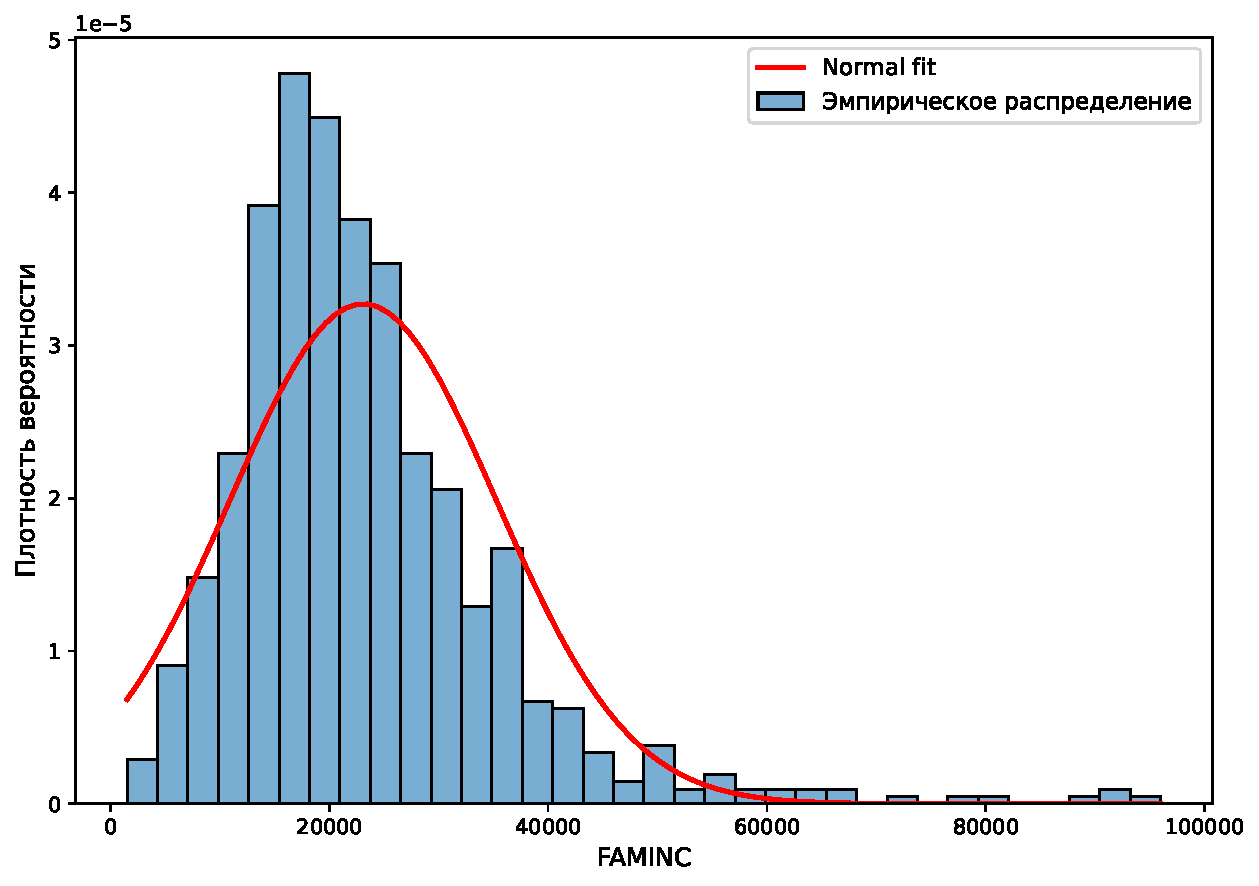
\includegraphics[keepaspectratio]{list21-LPM_files/figure-pdf/fig-faminc-dist-output-1.pdf}}

}

\caption{\label{fig-faminc-dist}Гистограмма распределения дохода семьи
(\(\textrm{FAMINC}\)) с наложением нормальной кривой плотности.}

\end{figure}%

Нарисуем гистограмму \(\log(\textrm{FAMINC})\) с наложенной кривой
нормального распределения

\begin{figure}

\centering{

\pandocbounded{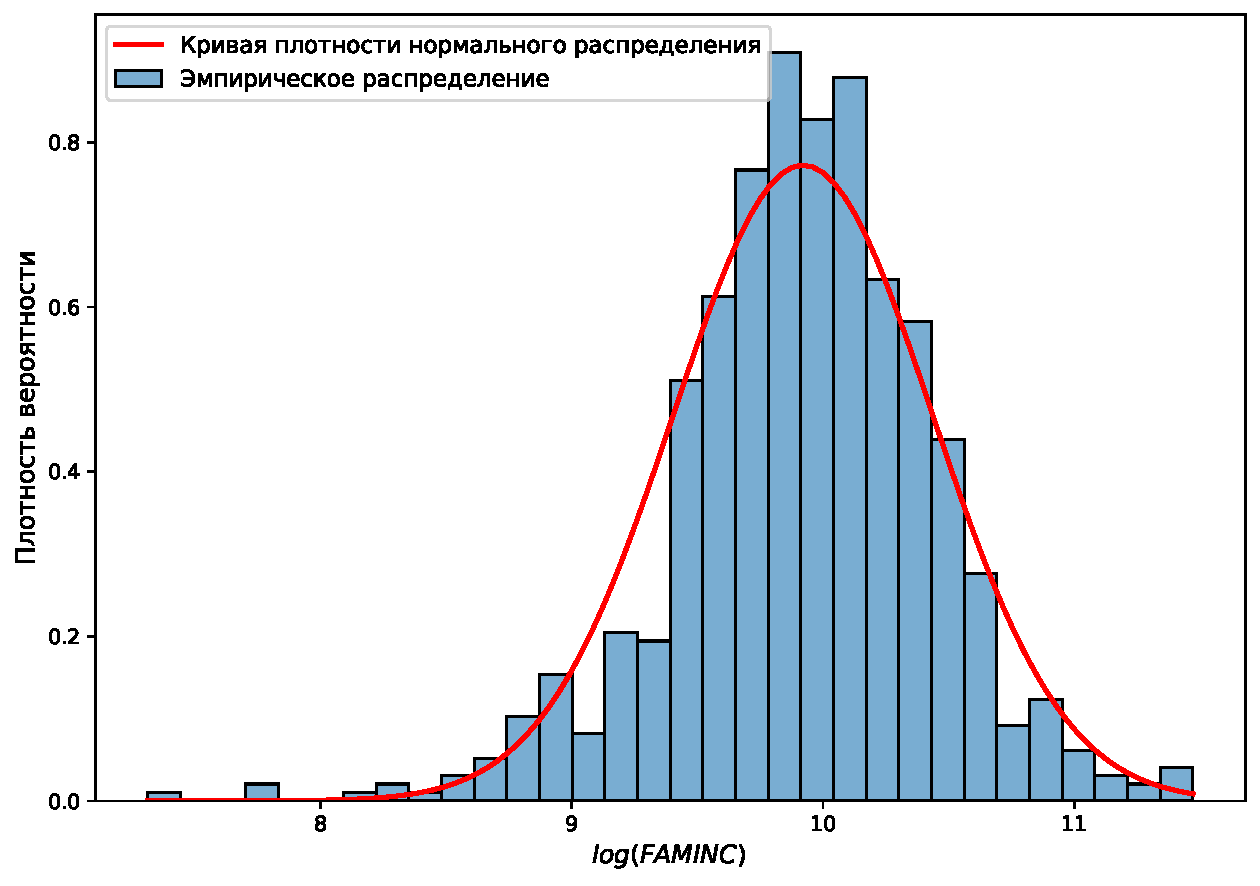
\includegraphics[keepaspectratio]{list21-LPM_files/figure-pdf/fig-log-faminc-output-1.pdf}}

}

\caption{\label{fig-log-faminc}Гистограмма логарифмированного дохода
семьи с наложением нормальной кривой плотности.}

\end{figure}%

\section{t-тест}\label{t-ux442ux435ux441ux442}

\subsection{approve equation \#1}\label{approve-equation-1-1}

Для датасета \texttt{loanapp} рассмотрим регрессию \textbf{approve на
mortno, unem, dep, male, married, yjob, self}

Оцените модель на данных и укажите (робастные) коэффициенты подогнанной
модели. \textbf{Ответ округлите до 3-х десятичных знаков.}

Ответ:

{\def\LTcaptype{none} % do not increment counter
\begin{longtable}[]{@{}lr@{}}
\toprule\noalign{}
Переменная & Оценка (HC3) \\
\midrule\noalign{}
\endhead
\bottomrule\noalign{}
\endlastfoot
Intercept & 0.864 \\
mortno & 0.073 \\
unem & -0.006 \\
dep & -0.018 \\
male & 0.002 \\
married & 0.046 \\
yjob & -0.001 \\
self & -0.036 \\
\end{longtable}
}

Модель была подогнана по 1971 наблюдению. {Уровень значимости 1\%}

Вычислите критическое значения для \(t\)-теста. \textbf{Ответ округлите
до 3-х десятичных знаков.}

\begin{tcolorbox}[enhanced jigsaw, arc=.35mm, bottomrule=.15mm, bottomtitle=1mm, breakable, colback=white, colbacktitle=quarto-callout-note-color!10!white, colframe=quarto-callout-note-color-frame, coltitle=black, left=2mm, leftrule=.75mm, opacityback=0, opacitybacktitle=0.6, rightrule=.15mm, title=\textcolor{quarto-callout-note-color}{\faInfo}\hspace{0.5em}{Критическое значение}, titlerule=0mm, toprule=.15mm, toptitle=1mm]

\(t_{crit} = 2.578\)

\end{tcolorbox}

\textbf{Укажите результаты робастного и неробастного \(t\)-теста. Ответ
округлите до 3-х десятичных знаков.}

\textbf{Результаты \(t\)-теста для коэффициентов (неробастные
стандартные ошибки, s.e.)}

{\def\LTcaptype{none} % do not increment counter
\begin{longtable}[]{@{}lrrrrl@{}}
\toprule\noalign{}
& Coef. & Std.Err. & t-value & p-value & Signif. \\
\midrule\noalign{}
\endhead
\bottomrule\noalign{}
\endlastfoot
Intercept & 0.864 & 0.022 & 39.444 & 0 & \\
mortno & 0.073 & 0.016 & 4.578 & 0 & *** \\
unem & -0.006 & 0.003 & -1.858 & 0.063 & * \\
dep & -0.018 & 0.007 & -2.57 & 0.01 & ** \\
male & 0.002 & 0.02 & 0.094 & 0.925 & \\
married & 0.046 & 0.018 & 2.604 & 0.009 & *** \\
yjob & -0.001 & 0.007 & -0.099 & 0.921 & \\
self & -0.036 & 0.022 & -1.621 & 0.105 & \\
\end{longtable}
}

\emph{Signif. codes:} \texttt{***} \(p<0.01\), \texttt{**} \(p<0.05\),
\texttt{*} \(p<0.1\)

Какие коэффициенты значимы?

\begin{tcolorbox}[enhanced jigsaw, arc=.35mm, bottomrule=.15mm, bottomtitle=1mm, breakable, colback=white, colbacktitle=quarto-callout-note-color!10!white, colframe=quarto-callout-note-color-frame, coltitle=black, left=2mm, leftrule=.75mm, opacityback=0, opacitybacktitle=0.6, rightrule=.15mm, title=\textcolor{quarto-callout-note-color}{\faInfo}\hspace{0.5em}{Коэффициенты, значимые на уровне 1\% (по классическим стандартным
ошибкам)}, titlerule=0mm, toprule=.15mm, toptitle=1mm]

\texttt{mortno}, \texttt{married}

\end{tcolorbox}

\textbf{Результаты \(t\)-теста для коэффициентов (робастные стандартные
ошибки, HC3-s.e.): }

{\def\LTcaptype{none} % do not increment counter
\begin{longtable}[]{@{}lrrrrl@{}}
\toprule\noalign{}
& Coef. & Std.Err. & t-value & p-value & Signif. \\
\midrule\noalign{}
\endhead
\bottomrule\noalign{}
\endlastfoot
Intercept & 0.864 & 0.023 & 37.135 & 0 & \\
mortno & 0.073 & 0.015 & 4.886 & 0 & *** \\
unem & -0.006 & 0.004 & -1.605 & 0.108 & \\
dep & -0.018 & 0.008 & -2.429 & 0.015 & ** \\
male & 0.002 & 0.021 & 0.089 & 0.929 & \\
married & 0.046 & 0.019 & 2.458 & 0.014 & ** \\
yjob & -0.001 & 0.006 & -0.107 & 0.915 & \\
self & -0.036 & 0.025 & -1.464 & 0.143 & \\
\end{longtable}
}

\emph{Signif. codes:} \texttt{***} \(p<0.01\), \texttt{**} \(p<0.05\),
\texttt{*} \(p<0.1\)

Какие коэффициенты значимы?

\begin{tcolorbox}[enhanced jigsaw, arc=.35mm, bottomrule=.15mm, bottomtitle=1mm, breakable, colback=white, colbacktitle=quarto-callout-note-color!10!white, colframe=quarto-callout-note-color-frame, coltitle=black, left=2mm, leftrule=.75mm, opacityback=0, opacitybacktitle=0.6, rightrule=.15mm, title=\textcolor{quarto-callout-note-color}{\faInfo}\hspace{0.5em}{Коэффициенты, значимые на уровне 1\% (по робастным стандартным ошибкам
HC3)}, titlerule=0mm, toprule=.15mm, toptitle=1mm]

\texttt{mortno}

\end{tcolorbox}

\begin{tcolorbox}[enhanced jigsaw, arc=.35mm, bottomrule=.15mm, bottomtitle=1mm, breakable, colback=white, colbacktitle=quarto-callout-note-color!10!white, colframe=quarto-callout-note-color-frame, coltitle=black, left=2mm, leftrule=.75mm, opacityback=0, opacitybacktitle=0.6, rightrule=.15mm, title=\textcolor{quarto-callout-note-color}{\faInfo}\hspace{0.5em}{Расшифровка кодов статистической значимости (Signif. codes)}, titlerule=0mm, toprule=.15mm, toptitle=1mm]

В таблицах регрессионного анализа звездочками традиционно обозначается
\(p\)-значение (p-value) для каждого коэффициента. Чем меньше
\(p\)-значение, тем сильнее статистические доказательства против нулевой
гипотезы (\(H_0\)), согласно которой данный фактор не влияет на
зависимую переменную (истинный коэффициент равен нулю).

\begin{itemize}
\tightlist
\item
  \texttt{***} : \textbf{\(p < 0.01\)} (от 0 до 0.01) --- \emph{высокая
  значимость}. Нулевая гипотеза отвергается на уровне значимости 1\%.
\item
  \texttt{**} : \textbf{\(0.01 \le p < 0.05\)} --- \emph{стандартная
  значимость}. Коэффициент значим на 5\% уровне. Это самый
  распространенный порог для подтверждения гипотез в большинстве
  исследований.
\item
  \texttt{*} : \textbf{\(0.05 \le p < 0.1\)} --- \emph{маргинальная
  (слабая) значимость}. Коэффициент значим лишь на 10\% уровне. В
  строгих моделях предиктор признают незначимым, но иногда
  интерпретируют как «статистическую тенденцию».
\item
  \texttt{} (пустое место) : \textbf{\(p \ge 0.1\)} (от 0.1 до 1) ---
  \emph{статистически не значимо}. У нас нет достаточных оснований
  утверждать, что переменная оказывает влияние на результат.
\end{itemize}

\end{tcolorbox}

\subsection{approve equation \#2}\label{approve-equation-2-1}

Для датасета \texttt{loanapp} рассмотрим регрессию \textbf{approve на
appinc, I(appinc ** 2), mortno, unem, dep, male, married, yjob, self}

Оцените модель на данных и укажите (робастные) коэффициенты подогнанной
модели. \textbf{Ответ округлите до 3-х десятичных знаков.}

Ответ:

{\def\LTcaptype{none} % do not increment counter
\begin{longtable}[]{@{}lr@{}}
\toprule\noalign{}
Переменная & Оценка (HC3) \\
\midrule\noalign{}
\endhead
\bottomrule\noalign{}
\endlastfoot
Intercept & 0.842 \\
appinc & 0.001 \\
I(appinc ** 2) & -0 \\
mortno & 0.066 \\
unem & -0.006 \\
dep & -0.017 \\
male & -0.003 \\
married & 0.043 \\
yjob & -0.001 \\
self & -0.04 \\
\end{longtable}
}

Модель была подогнана по 1971 наблюдению. {Уровень значимости 1\%}

Вычислите критическое значения для \(t\)-теста. \textbf{Ответ округлите
до 3-х десятичных знаков.}

Ответ:

\begin{tcolorbox}[enhanced jigsaw, arc=.35mm, bottomrule=.15mm, bottomtitle=1mm, breakable, colback=white, colbacktitle=quarto-callout-note-color!10!white, colframe=quarto-callout-note-color-frame, coltitle=black, left=2mm, leftrule=.75mm, opacityback=0, opacitybacktitle=0.6, rightrule=.15mm, title=\textcolor{quarto-callout-note-color}{\faInfo}\hspace{0.5em}{Критическое значение}, titlerule=0mm, toprule=.15mm, toptitle=1mm]

\(t_{crit} = 2.578\)

\end{tcolorbox}

\textbf{Укажите результаты робастного и неробастного \(t\)-теста. Ответ
округлите до 3-х десятичных знаков.}

\textbf{Результаты \(t\)-теста для коэффициентов (неробастные
стандартные ошибки, s.e.)}

{\def\LTcaptype{none} % do not increment counter
\begin{longtable}[]{@{}
  >{\raggedright\arraybackslash}p{(\linewidth - 10\tabcolsep) * \real{0.2286}}
  >{\raggedleft\arraybackslash}p{(\linewidth - 10\tabcolsep) * \real{0.1286}}
  >{\raggedleft\arraybackslash}p{(\linewidth - 10\tabcolsep) * \real{0.1714}}
  >{\raggedleft\arraybackslash}p{(\linewidth - 10\tabcolsep) * \real{0.1571}}
  >{\raggedleft\arraybackslash}p{(\linewidth - 10\tabcolsep) * \real{0.1571}}
  >{\raggedright\arraybackslash}p{(\linewidth - 10\tabcolsep) * \real{0.1571}}@{}}
\toprule\noalign{}
\begin{minipage}[b]{\linewidth}\raggedright
\end{minipage} & \begin{minipage}[b]{\linewidth}\raggedleft
Coef.
\end{minipage} & \begin{minipage}[b]{\linewidth}\raggedleft
Std.Err.
\end{minipage} & \begin{minipage}[b]{\linewidth}\raggedleft
t-value
\end{minipage} & \begin{minipage}[b]{\linewidth}\raggedleft
p-value
\end{minipage} & \begin{minipage}[b]{\linewidth}\raggedright
Signif.
\end{minipage} \\
\midrule\noalign{}
\endhead
\bottomrule\noalign{}
\endlastfoot
Intercept & 0.842 & 0.025 & 33.3 & 0 & \\
appinc & 0.001 & 0 & 2.082 & 0.037 & ** \\
I(appinc ** 2) & -0 & 0 & -2.803 & 0.005 & *** \\
mortno & 0.066 & 0.016 & 4.029 & 0 & *** \\
unem & -0.006 & 0.003 & -1.757 & 0.079 & * \\
dep & -0.017 & 0.007 & -2.374 & 0.018 & ** \\
male & -0.003 & 0.02 & -0.142 & 0.887 & \\
married & 0.043 & 0.018 & 2.449 & 0.014 & ** \\
yjob & -0.001 & 0.007 & -0.132 & 0.895 & \\
self & -0.04 & 0.023 & -1.786 & 0.074 & * \\
\end{longtable}
}

\emph{Signif. codes:} \texttt{***} \(p<0.01\), \texttt{**} \(p<0.05\),
\texttt{*} \(p<0.1\)

Какие коэффициенты значимы?

\begin{tcolorbox}[enhanced jigsaw, arc=.35mm, bottomrule=.15mm, bottomtitle=1mm, breakable, colback=white, colbacktitle=quarto-callout-note-color!10!white, colframe=quarto-callout-note-color-frame, coltitle=black, left=2mm, leftrule=.75mm, opacityback=0, opacitybacktitle=0.6, rightrule=.15mm, title=\textcolor{quarto-callout-note-color}{\faInfo}\hspace{0.5em}{Коэффициенты, значимые на уровне 1\% (по классическим стандартным
ошибкам)}, titlerule=0mm, toprule=.15mm, toptitle=1mm]

\texttt{I(appinc\ **\ 2)}, \texttt{mortno}

\end{tcolorbox}

\textbf{Результаты \(t\)-теста для коэффициентов (робастные стандартные
ошибки, HC3-s.e.): }

{\def\LTcaptype{none} % do not increment counter
\begin{longtable}[]{@{}
  >{\raggedright\arraybackslash}p{(\linewidth - 10\tabcolsep) * \real{0.2286}}
  >{\raggedleft\arraybackslash}p{(\linewidth - 10\tabcolsep) * \real{0.1286}}
  >{\raggedleft\arraybackslash}p{(\linewidth - 10\tabcolsep) * \real{0.1714}}
  >{\raggedleft\arraybackslash}p{(\linewidth - 10\tabcolsep) * \real{0.1571}}
  >{\raggedleft\arraybackslash}p{(\linewidth - 10\tabcolsep) * \real{0.1571}}
  >{\raggedright\arraybackslash}p{(\linewidth - 10\tabcolsep) * \real{0.1571}}@{}}
\toprule\noalign{}
\begin{minipage}[b]{\linewidth}\raggedright
\end{minipage} & \begin{minipage}[b]{\linewidth}\raggedleft
Coef.
\end{minipage} & \begin{minipage}[b]{\linewidth}\raggedleft
Std.Err.
\end{minipage} & \begin{minipage}[b]{\linewidth}\raggedleft
t-value
\end{minipage} & \begin{minipage}[b]{\linewidth}\raggedleft
p-value
\end{minipage} & \begin{minipage}[b]{\linewidth}\raggedright
Signif.
\end{minipage} \\
\midrule\noalign{}
\endhead
\bottomrule\noalign{}
\endlastfoot
Intercept & 0.842 & 0.027 & 31.003 & 0 & \\
appinc & 0.001 & 0 & 1.958 & 0.05 & * \\
I(appinc ** 2) & -0 & 0 & -2.374 & 0.018 & ** \\
mortno & 0.066 & 0.015 & 4.321 & 0 & *** \\
unem & -0.006 & 0.004 & -1.515 & 0.13 & \\
dep & -0.017 & 0.007 & -2.28 & 0.023 & ** \\
male & -0.003 & 0.021 & -0.135 & 0.893 & \\
married & 0.043 & 0.019 & 2.309 & 0.021 & ** \\
yjob & -0.001 & 0.006 & -0.14 & 0.889 & \\
self & -0.04 & 0.025 & -1.602 & 0.109 & \\
\end{longtable}
}

\emph{Signif. codes:} \texttt{***} \(p<0.01\), \texttt{**} \(p<0.05\),
\texttt{*} \(p<0.1\)

Какие коэффициенты значимы?

\begin{tcolorbox}[enhanced jigsaw, arc=.35mm, bottomrule=.15mm, bottomtitle=1mm, breakable, colback=white, colbacktitle=quarto-callout-note-color!10!white, colframe=quarto-callout-note-color-frame, coltitle=black, left=2mm, leftrule=.75mm, opacityback=0, opacitybacktitle=0.6, rightrule=.15mm, title=\textcolor{quarto-callout-note-color}{\faInfo}\hspace{0.5em}{Коэффициенты, значимые на уровне 1\% (по робастным стандартным ошибкам
HC3)}, titlerule=0mm, toprule=.15mm, toptitle=1mm]

\texttt{mortno}

\end{tcolorbox}

\subsection{labour force equation \#1}\label{labour-force-equation-1-1}

Для датасета \texttt{TableF5-1} рассмотрим регрессию \textbf{LFP на WA,
I(WA ** 2), WE, KL6, K618, CIT, UN, np.log(FAMINC)}

Оцените модель на данных и укажите (робастные) коэффициенты подогнанной
модели. \textbf{Ответ округлите до 3-х десятичных знаков.}

Ответ:

{\def\LTcaptype{none} % do not increment counter
\begin{longtable}[]{@{}lr@{}}
\toprule\noalign{}
Переменная & Оценка (HC3) \\
\midrule\noalign{}
\endhead
\bottomrule\noalign{}
\endlastfoot
Intercept & -0.321 \\
WA & 0.008 \\
I(WA ** 2) & -0 \\
WE & 0.038 \\
KL6 & -0.296 \\
K618 & -0.021 \\
CIT & -0.048 \\
UN & -0.004 \\
np.log(FAMINC) & 0.072 \\
\end{longtable}
}

Модель была подогнана по 753 наблюдению. {Уровень значимости 1\%}

Вычислите критическое значения для \(t\)-теста. \textbf{Ответ округлите
до 3-х десятичных знаков.}

Ответ:

\begin{tcolorbox}[enhanced jigsaw, arc=.35mm, bottomrule=.15mm, bottomtitle=1mm, breakable, colback=white, colbacktitle=quarto-callout-note-color!10!white, colframe=quarto-callout-note-color-frame, coltitle=black, left=2mm, leftrule=.75mm, opacityback=0, opacitybacktitle=0.6, rightrule=.15mm, title=\textcolor{quarto-callout-note-color}{\faInfo}\hspace{0.5em}{Критическое значение}, titlerule=0mm, toprule=.15mm, toptitle=1mm]

\(t_{crit} = 2.582\)

\end{tcolorbox}

\textbf{Укажите результаты робастного и неробастного \(t\)-теста. Ответ
округлите до 3-х десятичных знаков.}

\textbf{Результаты \(t\)-теста для коэффициентов (неробастные
стандартные ошибки, s.e.)}

{\def\LTcaptype{none} % do not increment counter
\begin{longtable}[]{@{}
  >{\raggedright\arraybackslash}p{(\linewidth - 10\tabcolsep) * \real{0.2286}}
  >{\raggedleft\arraybackslash}p{(\linewidth - 10\tabcolsep) * \real{0.1286}}
  >{\raggedleft\arraybackslash}p{(\linewidth - 10\tabcolsep) * \real{0.1714}}
  >{\raggedleft\arraybackslash}p{(\linewidth - 10\tabcolsep) * \real{0.1571}}
  >{\raggedleft\arraybackslash}p{(\linewidth - 10\tabcolsep) * \real{0.1571}}
  >{\raggedright\arraybackslash}p{(\linewidth - 10\tabcolsep) * \real{0.1571}}@{}}
\toprule\noalign{}
\begin{minipage}[b]{\linewidth}\raggedright
\end{minipage} & \begin{minipage}[b]{\linewidth}\raggedleft
Coef.
\end{minipage} & \begin{minipage}[b]{\linewidth}\raggedleft
Std.Err.
\end{minipage} & \begin{minipage}[b]{\linewidth}\raggedleft
t-value
\end{minipage} & \begin{minipage}[b]{\linewidth}\raggedleft
p-value
\end{minipage} & \begin{minipage}[b]{\linewidth}\raggedright
Signif.
\end{minipage} \\
\midrule\noalign{}
\endhead
\bottomrule\noalign{}
\endlastfoot
Intercept & -0.321 & 0.592 & -0.542 & 0.588 & \\
WA & 0.008 & 0.025 & 0.305 & 0.76 & \\
I(WA ** 2) & -0 & 0 & -0.847 & 0.398 & \\
WE & 0.038 & 0.008 & 4.574 & 0 & *** \\
KL6 & -0.296 & 0.037 & -8.011 & 0 & *** \\
K618 & -0.021 & 0.015 & -1.434 & 0.152 & \\
CIT & -0.048 & 0.038 & -1.283 & 0.2 & \\
UN & -0.004 & 0.006 & -0.647 & 0.518 & \\
np.log(FAMINC) & 0.072 & 0.037 & 1.965 & 0.05 & ** \\
\end{longtable}
}

\emph{Signif. codes:} \texttt{***} \(p<0.01\), \texttt{**} \(p<0.05\),
\texttt{*} \(p<0.1\)

Какие коэффициенты значимы?

\begin{tcolorbox}[enhanced jigsaw, arc=.35mm, bottomrule=.15mm, bottomtitle=1mm, breakable, colback=white, colbacktitle=quarto-callout-note-color!10!white, colframe=quarto-callout-note-color-frame, coltitle=black, left=2mm, leftrule=.75mm, opacityback=0, opacitybacktitle=0.6, rightrule=.15mm, title=\textcolor{quarto-callout-note-color}{\faInfo}\hspace{0.5em}{Коэффициенты, значимые на уровне 1\% (по классическим стандартным
ошибкам)}, titlerule=0mm, toprule=.15mm, toptitle=1mm]

\texttt{WE}, \texttt{KL6}

\end{tcolorbox}

\textbf{Результаты \(t\)-теста для коэффициентов (робастные стандартные
ошибки, HC3-s.e.): }

{\def\LTcaptype{none} % do not increment counter
\begin{longtable}[]{@{}
  >{\raggedright\arraybackslash}p{(\linewidth - 10\tabcolsep) * \real{0.2286}}
  >{\raggedleft\arraybackslash}p{(\linewidth - 10\tabcolsep) * \real{0.1286}}
  >{\raggedleft\arraybackslash}p{(\linewidth - 10\tabcolsep) * \real{0.1714}}
  >{\raggedleft\arraybackslash}p{(\linewidth - 10\tabcolsep) * \real{0.1571}}
  >{\raggedleft\arraybackslash}p{(\linewidth - 10\tabcolsep) * \real{0.1571}}
  >{\raggedright\arraybackslash}p{(\linewidth - 10\tabcolsep) * \real{0.1571}}@{}}
\toprule\noalign{}
\begin{minipage}[b]{\linewidth}\raggedright
\end{minipage} & \begin{minipage}[b]{\linewidth}\raggedleft
Coef.
\end{minipage} & \begin{minipage}[b]{\linewidth}\raggedleft
Std.Err.
\end{minipage} & \begin{minipage}[b]{\linewidth}\raggedleft
t-value
\end{minipage} & \begin{minipage}[b]{\linewidth}\raggedleft
p-value
\end{minipage} & \begin{minipage}[b]{\linewidth}\raggedright
Signif.
\end{minipage} \\
\midrule\noalign{}
\endhead
\bottomrule\noalign{}
\endlastfoot
Intercept & -0.321 & 0.585 & -0.549 & 0.583 & \\
WA & 0.008 & 0.024 & 0.307 & 0.759 & \\
I(WA ** 2) & -0 & 0 & -0.843 & 0.399 & \\
WE & 0.038 & 0.008 & 4.736 & 0 & *** \\
KL6 & -0.296 & 0.034 & -8.763 & 0 & *** \\
K618 & -0.021 & 0.015 & -1.409 & 0.159 & \\
CIT & -0.048 & 0.037 & -1.3 & 0.193 & \\
UN & -0.004 & 0.006 & -0.633 & 0.527 & \\
np.log(FAMINC) & 0.072 & 0.038 & 1.921 & 0.055 & * \\
\end{longtable}
}

\emph{Signif. codes:} \texttt{***} \(p<0.01\), \texttt{**} \(p<0.05\),
\texttt{*} \(p<0.1\)

Какие коэффициенты значимы?

\begin{tcolorbox}[enhanced jigsaw, arc=.35mm, bottomrule=.15mm, bottomtitle=1mm, breakable, colback=white, colbacktitle=quarto-callout-note-color!10!white, colframe=quarto-callout-note-color-frame, coltitle=black, left=2mm, leftrule=.75mm, opacityback=0, opacitybacktitle=0.6, rightrule=.15mm, title=\textcolor{quarto-callout-note-color}{\faInfo}\hspace{0.5em}{Коэффициенты, значимые на уровне 1\% (по робастным стандартным ошибкам
HC3)}, titlerule=0mm, toprule=.15mm, toptitle=1mm]

\texttt{WE}, \texttt{KL6}

\end{tcolorbox}

\subsection{labour force equation \#2}\label{labour-force-equation-2-1}

Для датасета \texttt{TableF5-1} рассмотрим регрессию \textbf{LFP на WA,
WE, CIT, UN, np.log(FAMINC)}

Оцените модель на данных и укажите (робастные) коэффициенты подогнанной
модели. \textbf{Ответ округлите до 3-х десятичных знаков.}

Ответ:

{\def\LTcaptype{none} % do not increment counter
\begin{longtable}[]{@{}lr@{}}
\toprule\noalign{}
Переменная & Оценка (HC3) \\
\midrule\noalign{}
\endhead
\bottomrule\noalign{}
\endlastfoot
Intercept & -0.536 \\
WA & -0.004 \\
WE & 0.033 \\
CIT & -0.048 \\
UN & -0.005 \\
np.log(FAMINC) & 0.094 \\
\end{longtable}
}

Модель была подогнана по 753 наблюдению. {Уровень значимости 5\%}

Вычислите критическое значения для \(t\)-теста. \textbf{Ответ округлите
до 3-х десятичных знаков.}

\begin{tcolorbox}[enhanced jigsaw, arc=.35mm, bottomrule=.15mm, bottomtitle=1mm, breakable, colback=white, colbacktitle=quarto-callout-note-color!10!white, colframe=quarto-callout-note-color-frame, coltitle=black, left=2mm, leftrule=.75mm, opacityback=0, opacitybacktitle=0.6, rightrule=.15mm, title=\textcolor{quarto-callout-note-color}{\faInfo}\hspace{0.5em}{Критическое значение}, titlerule=0mm, toprule=.15mm, toptitle=1mm]

\(t_{crit} = 1.963\)

\end{tcolorbox}

\textbf{Укажите результаты робастного и неробастного \(t\)-теста. Ответ
округлите до 3-х десятичных знаков.}

\textbf{Результаты \(t\)-теста для коэффициентов (неробастные
стандартные ошибки, s.e.)}

{\def\LTcaptype{none} % do not increment counter
\begin{longtable}[]{@{}
  >{\raggedright\arraybackslash}p{(\linewidth - 10\tabcolsep) * \real{0.2286}}
  >{\raggedleft\arraybackslash}p{(\linewidth - 10\tabcolsep) * \real{0.1286}}
  >{\raggedleft\arraybackslash}p{(\linewidth - 10\tabcolsep) * \real{0.1714}}
  >{\raggedleft\arraybackslash}p{(\linewidth - 10\tabcolsep) * \real{0.1571}}
  >{\raggedleft\arraybackslash}p{(\linewidth - 10\tabcolsep) * \real{0.1571}}
  >{\raggedright\arraybackslash}p{(\linewidth - 10\tabcolsep) * \real{0.1571}}@{}}
\toprule\noalign{}
\begin{minipage}[b]{\linewidth}\raggedright
\end{minipage} & \begin{minipage}[b]{\linewidth}\raggedleft
Coef.
\end{minipage} & \begin{minipage}[b]{\linewidth}\raggedleft
Std.Err.
\end{minipage} & \begin{minipage}[b]{\linewidth}\raggedleft
t-value
\end{minipage} & \begin{minipage}[b]{\linewidth}\raggedleft
p-value
\end{minipage} & \begin{minipage}[b]{\linewidth}\raggedright
Signif.
\end{minipage} \\
\midrule\noalign{}
\endhead
\bottomrule\noalign{}
\endlastfoot
Intercept & -0.536 & 0.36 & -1.488 & 0.137 & \\
WA & -0.004 & 0.002 & -1.668 & 0.096 & * \\
WE & 0.033 & 0.009 & 3.914 & 0 & *** \\
CIT & -0.048 & 0.039 & -1.217 & 0.224 & \\
UN & -0.005 & 0.006 & -0.868 & 0.386 & \\
np.log(FAMINC) & 0.094 & 0.038 & 2.449 & 0.015 & ** \\
\end{longtable}
}

\emph{Signif. codes:} \texttt{***} \(p<0.01\), \texttt{**} \(p<0.05\),
\texttt{*} \(p<0.1\)

Какие коэффициенты значимы?

\begin{tcolorbox}[enhanced jigsaw, arc=.35mm, bottomrule=.15mm, bottomtitle=1mm, breakable, colback=white, colbacktitle=quarto-callout-note-color!10!white, colframe=quarto-callout-note-color-frame, coltitle=black, left=2mm, leftrule=.75mm, opacityback=0, opacitybacktitle=0.6, rightrule=.15mm, title=\textcolor{quarto-callout-note-color}{\faInfo}\hspace{0.5em}{Коэффициенты, значимые на уровне 5\% (по классическим стандартным
ошибкам)}, titlerule=0mm, toprule=.15mm, toptitle=1mm]

\texttt{WE}, \texttt{np.log(FAMINC)}

\end{tcolorbox}

\textbf{Результаты \(t\)-теста для коэффициентов (робастные стандартные
ошибки, HC3-s.e.): }

{\def\LTcaptype{none} % do not increment counter
\begin{longtable}[]{@{}
  >{\raggedright\arraybackslash}p{(\linewidth - 10\tabcolsep) * \real{0.2286}}
  >{\raggedleft\arraybackslash}p{(\linewidth - 10\tabcolsep) * \real{0.1286}}
  >{\raggedleft\arraybackslash}p{(\linewidth - 10\tabcolsep) * \real{0.1714}}
  >{\raggedleft\arraybackslash}p{(\linewidth - 10\tabcolsep) * \real{0.1571}}
  >{\raggedleft\arraybackslash}p{(\linewidth - 10\tabcolsep) * \real{0.1571}}
  >{\raggedright\arraybackslash}p{(\linewidth - 10\tabcolsep) * \real{0.1571}}@{}}
\toprule\noalign{}
\begin{minipage}[b]{\linewidth}\raggedright
\end{minipage} & \begin{minipage}[b]{\linewidth}\raggedleft
Coef.
\end{minipage} & \begin{minipage}[b]{\linewidth}\raggedleft
Std.Err.
\end{minipage} & \begin{minipage}[b]{\linewidth}\raggedleft
t-value
\end{minipage} & \begin{minipage}[b]{\linewidth}\raggedleft
p-value
\end{minipage} & \begin{minipage}[b]{\linewidth}\raggedright
Signif.
\end{minipage} \\
\midrule\noalign{}
\endhead
\bottomrule\noalign{}
\endlastfoot
Intercept & -0.536 & 0.368 & -1.457 & 0.145 & \\
WA & -0.004 & 0.002 & -1.635 & 0.102 & \\
WE & 0.033 & 0.008 & 4.036 & 0 & *** \\
CIT & -0.048 & 0.039 & -1.212 & 0.226 & \\
UN & -0.005 & 0.006 & -0.855 & 0.392 & \\
np.log(FAMINC) & 0.094 & 0.04 & 2.351 & 0.019 & ** \\
\end{longtable}
}

\emph{Signif. codes:} \texttt{***} \(p<0.01\), \texttt{**} \(p<0.05\),
\texttt{*} \(p<0.1\)

Какие коэффициенты значимы?

\begin{tcolorbox}[enhanced jigsaw, arc=.35mm, bottomrule=.15mm, bottomtitle=1mm, breakable, colback=white, colbacktitle=quarto-callout-note-color!10!white, colframe=quarto-callout-note-color-frame, coltitle=black, left=2mm, leftrule=.75mm, opacityback=0, opacitybacktitle=0.6, rightrule=.15mm, title=\textcolor{quarto-callout-note-color}{\faInfo}\hspace{0.5em}{Коэффициенты, значимые на уровне 5\% (по робастным стандартным ошибкам
HC3)}, titlerule=0mm, toprule=.15mm, toptitle=1mm]

\texttt{WE}, \texttt{np.log(FAMINC)}

\end{tcolorbox}

\section{F-тест: значимость
регрессии}\label{f-ux442ux435ux441ux442-ux437ux43dux430ux447ux438ux43cux43eux441ux442ux44c-ux440ux435ux433ux440ux435ux441ux441ux438ux438}

\subsection{approve equation \#1}\label{approve-equation-1-2}

Для датасета \texttt{loanapp} рассмотрим регрессию \textbf{approve на
unem, male, yjob, self}

Результаты оценивания:

{\def\LTcaptype{none} % do not increment counter
\begin{longtable}[]{@{}lll@{}}
\toprule\noalign{}
& approve (OLS) & approve (HC3) \\
\midrule\noalign{}
\endhead
\bottomrule\noalign{}
\endlastfoot
unem & -0.007** & -0.007* \\
& (0.003) & (0.004) \\
male & 0.021 & 0.021 \\
& (0.019) & (0.020) \\
yjob & 0.001 & 0.001 \\
& (0.007) & (0.006) \\
self & -0.030 & -0.030 \\
& (0.022) & (0.025) \\
Intercept & 0.891*** & 0.891*** \\
& (0.021) & (0.023) \\
R-squared & 0.004 & 0.004 \\
R-squared Adj. & 0.002 & 0.002 \\
\end{longtable}
}

\emph{Signif. codes:} *** \(p<0.01\), ** \(p<0.05\), * \(p<0.1\)

{Зафиксируем уровень значимости 10\%.}

Тестируется значимость регрессии, т.е. гипотеза
\(H_0:\beta_{unem}=\beta_{male}=\beta_{yjob}=\beta_{self}=0\).

Вычислите критическое значение для гипотезы. \textbf{Ответ округлите до
3-х десятичных знаков.}

\begin{tcolorbox}[enhanced jigsaw, arc=.35mm, bottomrule=.15mm, bottomtitle=1mm, breakable, colback=white, colbacktitle=quarto-callout-note-color!10!white, colframe=quarto-callout-note-color-frame, coltitle=black, left=2mm, leftrule=.75mm, opacityback=0, opacitybacktitle=0.6, rightrule=.15mm, title=\textcolor{quarto-callout-note-color}{\faInfo}\hspace{0.5em}{Критическое значение}, titlerule=0mm, toprule=.15mm, toptitle=1mm]

\(F_{crit} = 1.948\)

\end{tcolorbox}

Получите результаты неробастного F-теста. \textbf{Ответ округлите до 3-х
десятичных знаков.}

{\def\LTcaptype{none} % do not increment counter
\begin{longtable}[]{@{}rr@{}}
\toprule\noalign{}
F-statistic & Prob(F-statistic) \\
\midrule\noalign{}
\endhead
\bottomrule\noalign{}
\endlastfoot
2.011 & 0.09 \\
\end{longtable}
}

Какой можно сделать вывод?

\begin{tcolorbox}[enhanced jigsaw, arc=.35mm, bottomrule=.15mm, bottomtitle=1mm, breakable, colback=white, colbacktitle=quarto-callout-tip-color!10!white, colframe=quarto-callout-tip-color-frame, coltitle=black, left=2mm, leftrule=.75mm, opacityback=0, opacitybacktitle=0.6, rightrule=.15mm, title=\textcolor{quarto-callout-tip-color}{\faLightbulb}\hspace{0.5em}{Вывод}, titlerule=0mm, toprule=.15mm, toptitle=1mm]

Регрессия \textbf{значима}.

\end{tcolorbox}

Получите результаты робастного F-теста. \textbf{Ответ округлите до 3-х
десятичных знаков.}

{\def\LTcaptype{none} % do not increment counter
\begin{longtable}[]{@{}rr@{}}
\toprule\noalign{}
F-statistic & Prob(F-statistic) \\
\midrule\noalign{}
\endhead
\bottomrule\noalign{}
\endlastfoot
1.667 & 0.155 \\
\end{longtable}
}

Какой можно сделать вывод?

\begin{tcolorbox}[enhanced jigsaw, arc=.35mm, bottomrule=.15mm, bottomtitle=1mm, breakable, colback=white, colbacktitle=quarto-callout-important-color!10!white, colframe=quarto-callout-important-color-frame, coltitle=black, left=2mm, leftrule=.75mm, opacityback=0, opacitybacktitle=0.6, rightrule=.15mm, title=\textcolor{quarto-callout-important-color}{\faExclamation}\hspace{0.5em}{Вывод}, titlerule=0mm, toprule=.15mm, toptitle=1mm]

Регрессия \textbf{незначима}.

\end{tcolorbox}

\subsection{approve equation \#2}\label{approve-equation-2-2}

Для датасета \texttt{loanapp} рассмотрим регрессию \textbf{approve на
appinc, I(appinc ** 2), mortno, dep}

{\def\LTcaptype{none} % do not increment counter
\begin{longtable}[]{@{}lll@{}}
\toprule\noalign{}
& OLS & HC3 \\
\midrule\noalign{}
\endhead
\bottomrule\noalign{}
\endlastfoot
unem & -0.007** & -0.007* \\
& (0.003) & (0.004) \\
Intercept & 0.856*** & 0.856*** \\
& (0.022) & (0.023) \\
appinc & 0.000** & 0.000** \\
& (0.000) & (0.000) \\
I(appinc ** 2) & -0.000*** & -0.000** \\
& (0.000) & (0.000) \\
mortno & 0.066*** & 0.066*** \\
& (0.016) & (0.015) \\
R-squared & 0.019 & 0.019 \\
R-squared Adj. & 0.017 & 0.017 \\
\end{longtable}
}

\emph{Signif. codes:} *** \(p<0.01\), ** \(p<0.05\), * \(p<0.1\)

{Зафиксируем уровень значимости 5\%.}

Тестируется значимость регрессии, т.е. гипотеза
\(H_0:\beta_{appinc}=\beta_{appinc^2}=\beta_{mortno}=\beta_{dep}=0\).

Вычислите критическое значение для гипотезы. \textbf{Ответ округлите до
3-х десятичных знаков.}

\begin{tcolorbox}[enhanced jigsaw, arc=.35mm, bottomrule=.15mm, bottomtitle=1mm, breakable, colback=white, colbacktitle=quarto-callout-note-color!10!white, colframe=quarto-callout-note-color-frame, coltitle=black, left=2mm, leftrule=.75mm, opacityback=0, opacitybacktitle=0.6, rightrule=.15mm, title=\textcolor{quarto-callout-note-color}{\faInfo}\hspace{0.5em}{Критическое значение}, titlerule=0mm, toprule=.15mm, toptitle=1mm]

\(F_{crit} = 2.376\)

\end{tcolorbox}

Получите результаты неробастного F-теста. \textbf{Ответ округлите до 3-х
десятичных знаков.}

{\def\LTcaptype{none} % do not increment counter
\begin{longtable}[]{@{}rr@{}}
\toprule\noalign{}
F-statistic & Prob(F-statistic) \\
\midrule\noalign{}
\endhead
\bottomrule\noalign{}
\endlastfoot
9.606 & 0 \\
\end{longtable}
}

Какой можно сделать вывод?

\begin{tcolorbox}[enhanced jigsaw, arc=.35mm, bottomrule=.15mm, bottomtitle=1mm, breakable, colback=white, colbacktitle=quarto-callout-tip-color!10!white, colframe=quarto-callout-tip-color-frame, coltitle=black, left=2mm, leftrule=.75mm, opacityback=0, opacitybacktitle=0.6, rightrule=.15mm, title=\textcolor{quarto-callout-tip-color}{\faLightbulb}\hspace{0.5em}{Вывод}, titlerule=0mm, toprule=.15mm, toptitle=1mm]

Регрессия \textbf{значима}.

\end{tcolorbox}

Получите результаты робастного F-теста. \textbf{Ответ округлите до 3-х
десятичных знаков.}

{\def\LTcaptype{none} % do not increment counter
\begin{longtable}[]{@{}rr@{}}
\toprule\noalign{}
F-statistic & Prob(F-statistic) \\
\midrule\noalign{}
\endhead
\bottomrule\noalign{}
\endlastfoot
9.13 & 0 \\
\end{longtable}
}

Какой можно сделать вывод?

\begin{tcolorbox}[enhanced jigsaw, arc=.35mm, bottomrule=.15mm, bottomtitle=1mm, breakable, colback=white, colbacktitle=quarto-callout-tip-color!10!white, colframe=quarto-callout-tip-color-frame, coltitle=black, left=2mm, leftrule=.75mm, opacityback=0, opacitybacktitle=0.6, rightrule=.15mm, title=\textcolor{quarto-callout-tip-color}{\faLightbulb}\hspace{0.5em}{Вывод}, titlerule=0mm, toprule=.15mm, toptitle=1mm]

Регрессия \textbf{значима}.

\end{tcolorbox}

\subsection{approve equation \#3}\label{approve-equation-3}

Для датасета \texttt{loanapp} рассмотрим регрессию \textbf{approve на
dep, male, married}

{\def\LTcaptype{none} % do not increment counter
\begin{longtable}[]{@{}lll@{}}
\toprule\noalign{}
& OLS & HC3 \\
\midrule\noalign{}
\endhead
\bottomrule\noalign{}
\endlastfoot
dep & -0.016** & -0.016** \\
& (0.007) & (0.008) \\
male & -0.002 & -0.002 \\
& (0.020) & (0.021) \\
married & 0.057*** & 0.057*** \\
& (0.018) & (0.019) \\
Intercept & 0.852*** & 0.852*** \\
& (0.018) & (0.019) \\
R-squared & 0.006 & 0.006 \\
R-squared Adj. & 0.005 & 0.005 \\
\end{longtable}
}

\emph{Signif. codes:} *** \(p<0.01\), ** \(p<0.05\), * \(p<0.1\)

{Зафиксируем уровень значимости 1\%.}

Тестируется значимость регрессии, т.е. гипотеза
\(H_0:\beta_{dep}=\beta_{male}=\beta_{married}=0\).

Вычислите критическое значение для гипотезы. \textbf{Ответ округлите до
3-х десятичных знаков.}

\begin{tcolorbox}[enhanced jigsaw, arc=.35mm, bottomrule=.15mm, bottomtitle=1mm, breakable, colback=white, colbacktitle=quarto-callout-note-color!10!white, colframe=quarto-callout-note-color-frame, coltitle=black, left=2mm, leftrule=.75mm, opacityback=0, opacitybacktitle=0.6, rightrule=.15mm, title=\textcolor{quarto-callout-note-color}{\faInfo}\hspace{0.5em}{Критическое значение}, titlerule=0mm, toprule=.15mm, toptitle=1mm]

\(F_{crit} = 3.792\)

\end{tcolorbox}

Получите результаты неробастного F-теста. \textbf{Ответ округлите до 3-х
десятичных знаков.}

{\def\LTcaptype{none} % do not increment counter
\begin{longtable}[]{@{}rr@{}}
\toprule\noalign{}
F-statistic & Prob(F-statistic) \\
\midrule\noalign{}
\endhead
\bottomrule\noalign{}
\endlastfoot
4.155 & 0.006 \\
\end{longtable}
}

Какой можно сделать вывод?

\begin{tcolorbox}[enhanced jigsaw, arc=.35mm, bottomrule=.15mm, bottomtitle=1mm, breakable, colback=white, colbacktitle=quarto-callout-tip-color!10!white, colframe=quarto-callout-tip-color-frame, coltitle=black, left=2mm, leftrule=.75mm, opacityback=0, opacitybacktitle=0.6, rightrule=.15mm, title=\textcolor{quarto-callout-tip-color}{\faLightbulb}\hspace{0.5em}{Вывод}, titlerule=0mm, toprule=.15mm, toptitle=1mm]

Регрессия \textbf{значима}.

\end{tcolorbox}

Получите результаты робастного F-теста. \textbf{Ответ округлите до 3-х
десятичных знаков.}

{\def\LTcaptype{none} % do not increment counter
\begin{longtable}[]{@{}rr@{}}
\toprule\noalign{}
F-statistic & Prob(F-statistic) \\
\midrule\noalign{}
\endhead
\bottomrule\noalign{}
\endlastfoot
3.724 & 0.011 \\
\end{longtable}
}

Какой можно сделать вывод?

\begin{tcolorbox}[enhanced jigsaw, arc=.35mm, bottomrule=.15mm, bottomtitle=1mm, breakable, colback=white, colbacktitle=quarto-callout-important-color!10!white, colframe=quarto-callout-important-color-frame, coltitle=black, left=2mm, leftrule=.75mm, opacityback=0, opacitybacktitle=0.6, rightrule=.15mm, title=\textcolor{quarto-callout-important-color}{\faExclamation}\hspace{0.5em}{Вывод}, titlerule=0mm, toprule=.15mm, toptitle=1mm]

Регрессия \textbf{незначима}.

\end{tcolorbox}

\section{F-тест: совместная
значимость}\label{f-ux442ux435ux441ux442-ux441ux43eux432ux43cux435ux441ux442ux43dux430ux44f-ux437ux43dux430ux447ux438ux43cux43eux441ux442ux44c}

\subsection{approve equation \#1}\label{approve-equation-1-3}

Для датасета \texttt{loanapp} рассмотрим регрессию \textbf{approve на
appinc, I(appinc ** 2), mortno, unem, dep, male, married, yjob, self}

{\def\LTcaptype{none} % do not increment counter
\begin{longtable}[]{@{}llll@{}}
\toprule\noalign{}
& Model 1 & Model 2 & Model 3 \\
\midrule\noalign{}
\endhead
\bottomrule\noalign{}
\endlastfoot
Dep. Variable & approve & approve & approve \\
appinc & 0.001* & & 0.001** \\
& (0.000) & & (0.000) \\
I(appinc ** 2) & -0.000** & & -0.000*** \\
& (0.000) & & (0.000) \\
mortno & 0.066*** & 0.073*** & 0.067*** \\
& (0.015) & (0.015) & (0.015) \\
unem & -0.006 & -0.006 & \\
& (0.004) & (0.004) & \\
dep & -0.017** & -0.018** & \\
& (0.007) & (0.008) & \\
male & -0.003 & 0.002 & 0.003 \\
& (0.021) & (0.021) & (0.020) \\
married & 0.043** & 0.046** & \\
& (0.019) & (0.019) & \\
yjob & -0.001 & -0.001 & -0.000 \\
& (0.006) & (0.006) & (0.006) \\
self & -0.040 & -0.036 & -0.050** \\
& (0.025) & (0.025) & (0.024) \\
Intercept & 0.842*** & 0.864*** & 0.824*** \\
& (0.027) & (0.023) & (0.023) \\
R-squared & 0.025 & 0.020 & 0.019 \\
R-squared Adj. & 0.021 & 0.017 & 0.016 \\
F-statistic & 5.032 & 5.849 & 6.172 \\
Nobs & 1971 & 1971 & 1971 \\
\end{longtable}
}

\emph{Signif. codes:} *** \(p<0.01\), ** \(p<0.05\), * \(p<0.1\)

\subsubsection{Гипотеза 1: значимость влияния
дохода}\label{ux433ux438ux43fux43eux442ux435ux437ux430-1-ux437ux43dux430ux447ux438ux43cux43eux441ux442ux44c-ux432ux43bux438ux44fux43dux438ux44f-ux434ux43eux445ux43eux434ux430}

Тестируется значимость влияния дохода, т.е. гипотеза
\(H_0:\beta_{appinc}=\beta_{appinc^2}=0\).

{Зафиксируем уровень значимости 5\%.}

Вычислите критическое значение для гипотезы. \textbf{Ответ округлите до
3-х десятичных знаков.}

\begin{tcolorbox}[enhanced jigsaw, arc=.35mm, bottomrule=.15mm, bottomtitle=1mm, breakable, colback=white, colbacktitle=quarto-callout-note-color!10!white, colframe=quarto-callout-note-color-frame, coltitle=black, left=2mm, leftrule=.75mm, opacityback=0, opacitybacktitle=0.6, rightrule=.15mm, title=\textcolor{quarto-callout-note-color}{\faInfo}\hspace{0.5em}{Критическое значение}, titlerule=0mm, toprule=.15mm, toptitle=1mm]

\(F_{crit} = 3.000\)

\end{tcolorbox}

Получите результаты неробастного F-теста. \textbf{Ответ округлите до 3-х
десятичных знаков.}

{\def\LTcaptype{none} % do not increment counter
\begin{longtable}[]{@{}rr@{}}
\toprule\noalign{}
F-statistic & Prob(F-statistic) \\
\midrule\noalign{}
\endhead
\bottomrule\noalign{}
\endlastfoot
5.149 & 0.006 \\
\end{longtable}
}

Какой можно сделать вывод?

\begin{tcolorbox}[enhanced jigsaw, arc=.35mm, bottomrule=.15mm, bottomtitle=1mm, breakable, colback=white, colbacktitle=quarto-callout-tip-color!10!white, colframe=quarto-callout-tip-color-frame, coltitle=black, left=2mm, leftrule=.75mm, opacityback=0, opacitybacktitle=0.6, rightrule=.15mm, title=\textcolor{quarto-callout-tip-color}{\faLightbulb}\hspace{0.5em}{Вывод}, titlerule=0mm, toprule=.15mm, toptitle=1mm]

Гипотеза \textbf{отвергается}.

\end{tcolorbox}

Получите результаты робастного F-теста. \textbf{Ответ округлите до 3-х
десятичных знаков.}

{\def\LTcaptype{none} % do not increment counter
\begin{longtable}[]{@{}rr@{}}
\toprule\noalign{}
F-statistic & Prob(F-statistic) \\
\midrule\noalign{}
\endhead
\bottomrule\noalign{}
\endlastfoot
2.961 & 0.052 \\
\end{longtable}
}

Какой можно сделать вывод?

\begin{tcolorbox}[enhanced jigsaw, arc=.35mm, bottomrule=.15mm, bottomtitle=1mm, breakable, colback=white, colbacktitle=quarto-callout-important-color!10!white, colframe=quarto-callout-important-color-frame, coltitle=black, left=2mm, leftrule=.75mm, opacityback=0, opacitybacktitle=0.6, rightrule=.15mm, title=\textcolor{quarto-callout-important-color}{\faExclamation}\hspace{0.5em}{Вывод}, titlerule=0mm, toprule=.15mm, toptitle=1mm]

Гипотеза \textbf{не отвергается}.

\end{tcolorbox}

\subsubsection{Гипотеза 2: совместная значимость unem, dep,
married}\label{ux433ux438ux43fux43eux442ux435ux437ux430-2-ux441ux43eux432ux43cux435ux441ux442ux43dux430ux44f-ux437ux43dux430ux447ux438ux43cux43eux441ux442ux44c-unem-dep-married}

Тестируется совместная значимость \texttt{unem}, \texttt{dep} и
\texttt{married}, т.е. гипотеза
\(H_0:\beta_{unem}=\beta_{dep}=\beta_{married}=0\).

{Зафиксируем уровень значимости 1\%.}

Вычислите критическое значение для гипотезы. \textbf{Ответ округлите до
3-х десятичных знаков.}

\begin{tcolorbox}[enhanced jigsaw, arc=.35mm, bottomrule=.15mm, bottomtitle=1mm, breakable, colback=white, colbacktitle=quarto-callout-note-color!10!white, colframe=quarto-callout-note-color-frame, coltitle=black, left=2mm, leftrule=.75mm, opacityback=0, opacitybacktitle=0.6, rightrule=.15mm, title=\textcolor{quarto-callout-note-color}{\faInfo}\hspace{0.5em}{Критическое значение}, titlerule=0mm, toprule=.15mm, toptitle=1mm]

\(F_{crit} = 3.792\)

\end{tcolorbox}

Получите результаты неробастного F-теста. \textbf{Ответ округлите до 3-х
десятичных знаков.}

{\def\LTcaptype{none} % do not increment counter
\begin{longtable}[]{@{}rr@{}}
\toprule\noalign{}
F-statistic & Prob(F-statistic) \\
\midrule\noalign{}
\endhead
\bottomrule\noalign{}
\endlastfoot
4.054 & 0.007 \\
\end{longtable}
}

Какой можно сделать вывод?

\begin{tcolorbox}[enhanced jigsaw, arc=.35mm, bottomrule=.15mm, bottomtitle=1mm, breakable, colback=white, colbacktitle=quarto-callout-tip-color!10!white, colframe=quarto-callout-tip-color-frame, coltitle=black, left=2mm, leftrule=.75mm, opacityback=0, opacitybacktitle=0.6, rightrule=.15mm, title=\textcolor{quarto-callout-tip-color}{\faLightbulb}\hspace{0.5em}{Вывод}, titlerule=0mm, toprule=.15mm, toptitle=1mm]

Гипотеза \textbf{отвергается} --- переменные \textbf{значимы совместно}.

\end{tcolorbox}

Получите результаты робастного F-теста. \textbf{Ответ округлите до 3-х
десятичных знаков.}

{\def\LTcaptype{none} % do not increment counter
\begin{longtable}[]{@{}rr@{}}
\toprule\noalign{}
F-statistic & Prob(F-statistic) \\
\midrule\noalign{}
\endhead
\bottomrule\noalign{}
\endlastfoot
3.469 & 0.016 \\
\end{longtable}
}

Какой можно сделать вывод?

\begin{tcolorbox}[enhanced jigsaw, arc=.35mm, bottomrule=.15mm, bottomtitle=1mm, breakable, colback=white, colbacktitle=quarto-callout-important-color!10!white, colframe=quarto-callout-important-color-frame, coltitle=black, left=2mm, leftrule=.75mm, opacityback=0, opacitybacktitle=0.6, rightrule=.15mm, title=\textcolor{quarto-callout-important-color}{\faExclamation}\hspace{0.5em}{Вывод}, titlerule=0mm, toprule=.15mm, toptitle=1mm]

Гипотеза \textbf{не отвергается} --- переменные \textbf{незначимы
совместно}.

\end{tcolorbox}

\section{Прогноз}\label{ux43fux440ux43eux433ux43dux43eux437}

\subsection{approve equation}\label{approve-equation}

Для датасета \texttt{loanapp} рассмотрим регрессию \textbf{approve на
mortno, unem, dep, married}

{\def\LTcaptype{none} % do not increment counter
\begin{longtable}[]{@{}ll@{}}
\toprule\noalign{}
& approve (HC3) \\
\midrule\noalign{}
\endhead
\bottomrule\noalign{}
\endlastfoot
mortno & 0.071*** \\
& (0.015) \\
unem & -0.007* \\
& (0.004) \\
dep & -0.019** \\
& (0.008) \\
married & 0.046*** \\
& (0.018) \\
Intercept & 0.865*** \\
& (0.020) \\
R-squared & 0.019 \\
R-squared Adj. & 0.017 \\
Nobs & 1971 \\
F-stat & 9.475 \\
Prob(F-stat) & 0.000 \\
\end{longtable}
}

\emph{Signif. codes:} *** \(p<0.01\), ** \(p<0.05\), * \(p<0.1\)

Рассмотрим трех людей с характеристиками

{\def\LTcaptype{none} % do not increment counter
\begin{longtable}[]{@{}rrrrr@{}}
\toprule\noalign{}
Человек & mortno & unem & dep & married \\
\midrule\noalign{}
\endhead
\bottomrule\noalign{}
\endlastfoot
1 & 1 & 3.2 & 0 & 1 \\
2 & 1 & 3.9 & 1 & 0 \\
3 & 0 & 1.8 & 0 & 1 \\
\end{longtable}
}

Вычислите прогноз для каждого человека по подогнанной модели.
\textbf{Ответ округлите до 3-х десятичных знаков.}

\textbf{Прогнозы вероятности одобрения кредита
\({\textrm P}(approve=1)\):}

{\def\LTcaptype{none} % do not increment counter
\begin{longtable}[]{@{}rr@{}}
\toprule\noalign{}
Человек & Прогноз \\
\midrule\noalign{}
\endhead
\bottomrule\noalign{}
\endlastfoot
1 & 0.959 \\
2 & 0.889 \\
3 & 0.898 \\
\end{longtable}
}

\subsection{labour force equation}\label{labour-force-equation}

Для датасета \texttt{TableF5-1} рассмотрим регрессию \textbf{LFP на WA,
I(WA ** 2), CIT, UN, np.log(FAMINC)}

{\def\LTcaptype{none} % do not increment counter
\begin{longtable}[]{@{}ll@{}}
\toprule\noalign{}
& LFP (HC3) \\
\midrule\noalign{}
\endhead
\bottomrule\noalign{}
\endlastfoot
WA & 0.042* \\
& (0.025) \\
I(WA ** 2) & -0.001* \\
& (0.000) \\
CIT & -0.039 \\
& (0.040) \\
UN & -0.004 \\
& (0.006) \\
np.log(FAMINC) & 0.140*** \\
& (0.037) \\
Intercept & -1.525** \\
& (0.600) \\
R-squared & 0.033 \\
R-squared Adj. & 0.027 \\
Nobs & 753 \\
F-stat & 4.994 \\
Prob(F-stat) & 0.000 \\
\end{longtable}
}

\emph{Signif. codes:} *** \(p<0.01\), ** \(p<0.05\), * \(p<0.1\)

Рассмотрим трех людей с характеристиками

{\def\LTcaptype{none} % do not increment counter
\begin{longtable}[]{@{}rrrrr@{}}
\toprule\noalign{}
Человек & WA & CIT & UN & FAMINC \\
\midrule\noalign{}
\endhead
\bottomrule\noalign{}
\endlastfoot
1 & 34 & 1 & 3 & 35000 \\
2 & 36 & 0 & 5 & 48500 \\
3 & 42 & 0 & 7.5 & 67800 \\
\end{longtable}
}

Вычислите прогноз для каждого человека по подогнанной модели.
\textbf{Ответ округлите до 3-х десятичных знаков.}

\textbf{Прогнозы вероятности участия в рабочей силе
\({\textrm P}(LFP=1)\):}

{\def\LTcaptype{none} % do not increment counter
\begin{longtable}[]{@{}rr@{}}
\toprule\noalign{}
Человек & Прогноз \\
\midrule\noalign{}
\endhead
\bottomrule\noalign{}
\endlastfoot
1 & 0.686 \\
2 & 0.771 \\
3 & 0.804 \\
\end{longtable}
}

\section{Вопросы адекватности
модели}\label{ux432ux43eux43fux440ux43eux441ux44b-ux430ux434ux435ux43aux432ux430ux442ux43dux43eux441ux442ux438-ux43cux43eux434ux435ux43bux438}

\subsection{approve equation}\label{approve-equation-4}

Для датасета \texttt{loanapp} рассмотрим регрессию \textbf{approve на
appinc, I(appinc ** 2), mortno, unem, dep, male, married, yjob, self}

\textbf{Доля правильных прогнозов (Accuracy) на обучающей выборке:}
\texttt{87.6\%}

\subsubsection{\texorpdfstring{Анализ переменной
\texttt{appinc}}{Анализ переменной appinc}}\label{ux430ux43dux430ux43bux438ux437-ux43fux435ux440ux435ux43cux435ux43dux43dux43eux439-appinc}

\pandocbounded{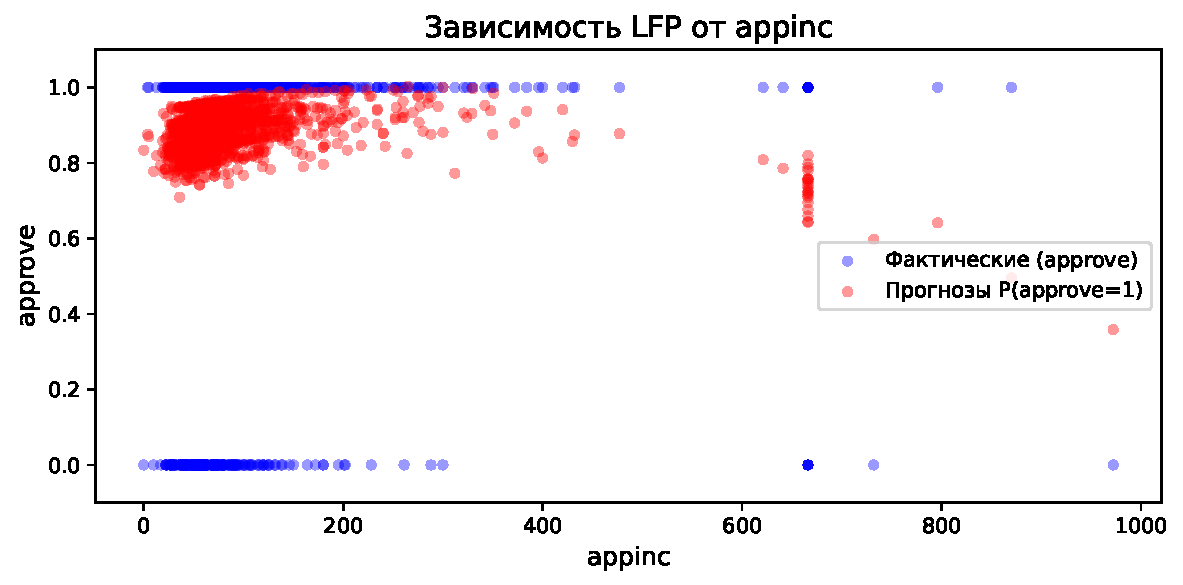
\includegraphics[keepaspectratio]{list21-LPM_files/figure-pdf/cell-74-output-3.pdf}}

\subsubsection{\texorpdfstring{Анализ переменной
\texttt{dep}}{Анализ переменной dep}}\label{ux430ux43dux430ux43bux438ux437-ux43fux435ux440ux435ux43cux435ux43dux43dux43eux439-dep}

\pandocbounded{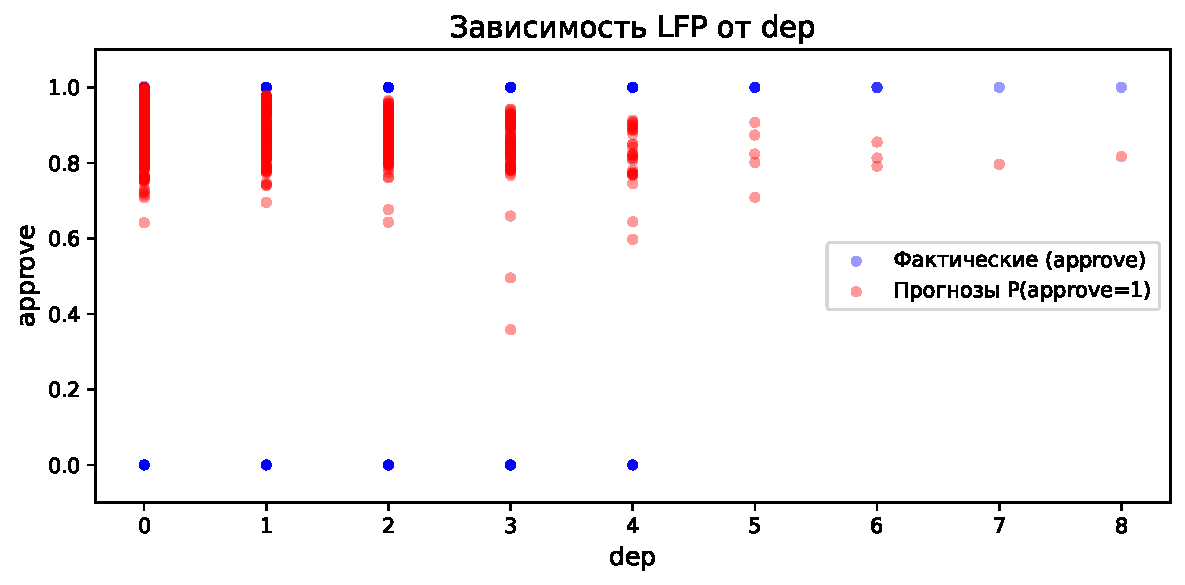
\includegraphics[keepaspectratio]{list21-LPM_files/figure-pdf/cell-74-output-5.pdf}}

\subsubsection{\texorpdfstring{Анализ переменной
\texttt{yjob}}{Анализ переменной yjob}}\label{ux430ux43dux430ux43bux438ux437-ux43fux435ux440ux435ux43cux435ux43dux43dux43eux439-yjob}

\pandocbounded{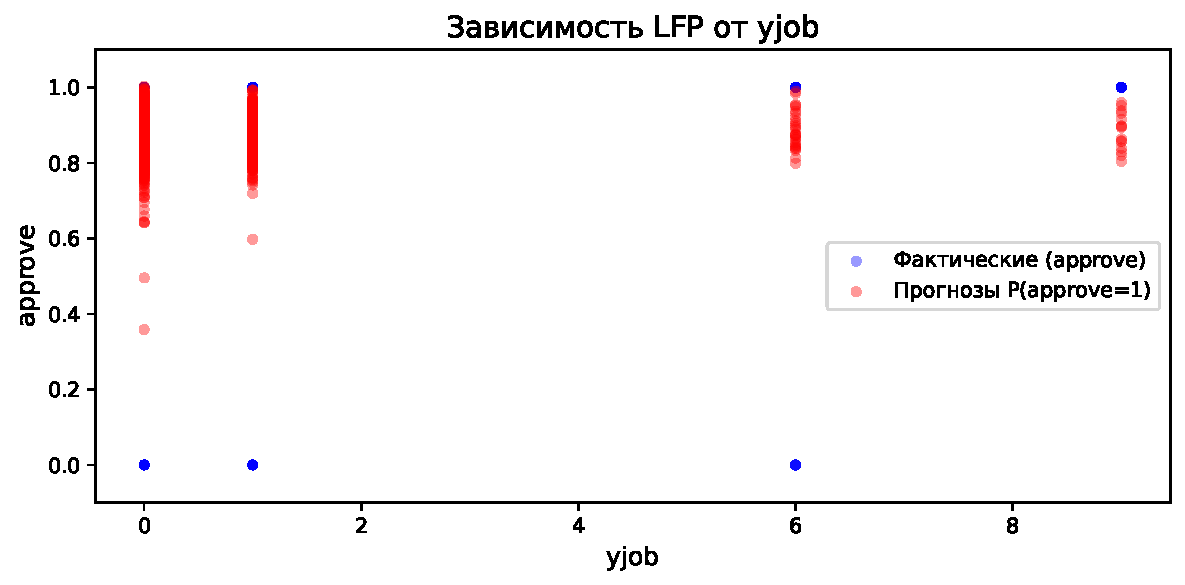
\includegraphics[keepaspectratio]{list21-LPM_files/figure-pdf/cell-74-output-7.pdf}}

\subsection{labour force equation}\label{labour-force-equation-3}

Для датасета \texttt{TableF5-1} рассмотрим регрессию \textbf{LFP на WA,
I(WA ** 2), WE, KL6, K618, CIT, UN, np.log(FAMINC)}

\textbf{Доля правильных прогнозов (Accuracy) на обучающей выборке:}
\texttt{66.4\%}

\subsubsection{\texorpdfstring{Анализ переменной
\texttt{WA}}{Анализ переменной WA}}\label{ux430ux43dux430ux43bux438ux437-ux43fux435ux440ux435ux43cux435ux43dux43dux43eux439-wa}

\pandocbounded{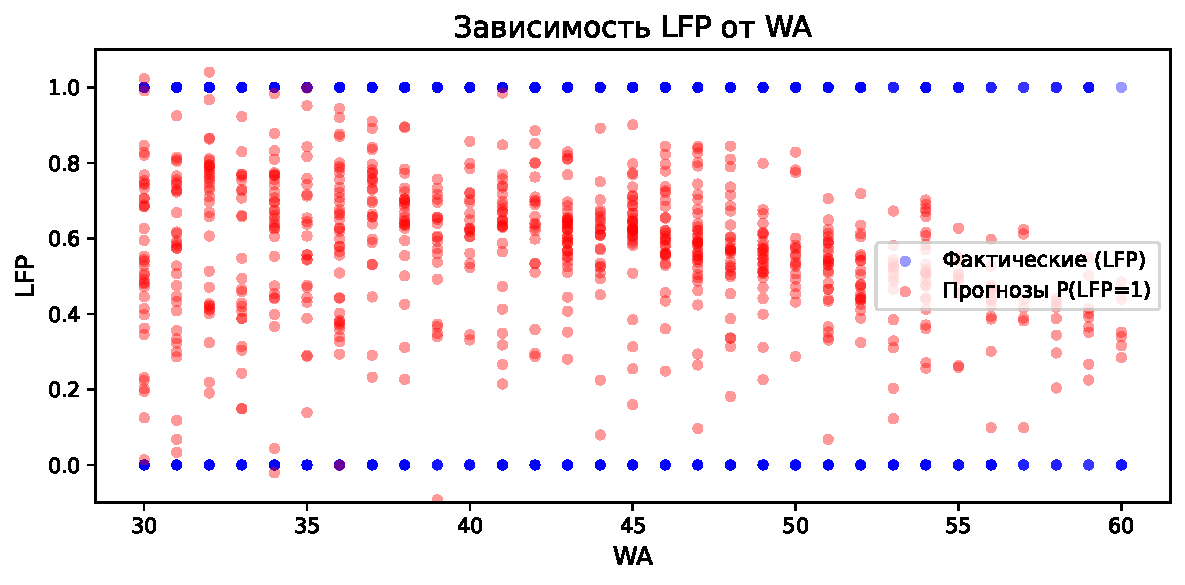
\includegraphics[keepaspectratio]{list21-LPM_files/figure-pdf/cell-75-output-3.pdf}}

\subsubsection{\texorpdfstring{Анализ переменной
\texttt{log(FAMINC)}}{Анализ переменной log(FAMINC)}}\label{ux430ux43dux430ux43bux438ux437-ux43fux435ux440ux435ux43cux435ux43dux43dux43eux439-logfaminc}

\pandocbounded{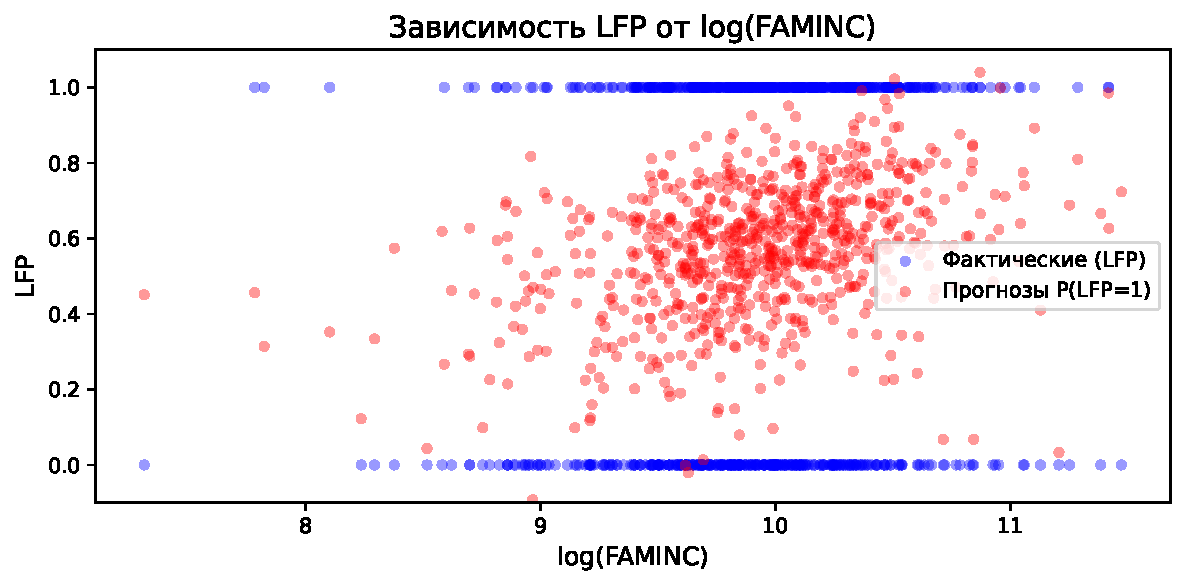
\includegraphics[keepaspectratio]{list21-LPM_files/figure-pdf/cell-75-output-5.pdf}}

\subsubsection{\texorpdfstring{Анализ переменной
\texttt{UN}}{Анализ переменной UN}}\label{ux430ux43dux430ux43bux438ux437-ux43fux435ux440ux435ux43cux435ux43dux43dux43eux439-un}

\pandocbounded{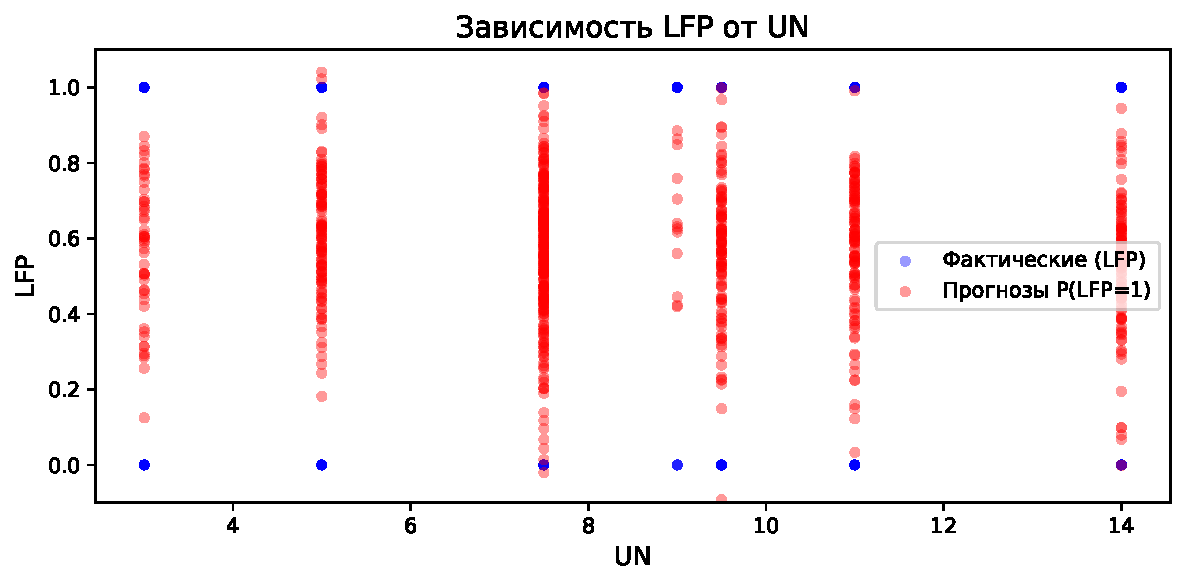
\includegraphics[keepaspectratio]{list21-LPM_files/figure-pdf/cell-75-output-7.pdf}}




\end{document}
